\documentclass{article}
\usepackage{graphicx} 
\usepackage{amsfonts,amsmath,amssymb}
\usepackage{array}
\usepackage{tabularray}
\usepackage[utf8]{inputenc}
\usepackage[T1]{fontenc}
\usepackage{csquotes}
\usepackage{alphabeta}
\usepackage{url}
\usepackage{hyperref}
\usepackage{esint}

\renewcommand{\figurename}{Γράφημα}

\begin{document}
\begin{table}[ht]
    \begin{tblr}{
        @{}X[l, valign=b]X[c, valign=b]X[r, valign=b]@{}
    }

    \hline
    % First line, course info
    \SetCell[c=2]{l}{[ΘΠ04] Παράλληλα Συστήματα} & & {2024-25} \\ 
    \hline
    {} & {} & {} \\

    % Title
    \SetCell[c=3]{c}{ \Large \textbf{Εργασία 1 - Προγραμματισμός με Pthreads} } \\
    {} & {} & {} \\

    % Name Surname, Student ID
    \hline
    \SetCell[c=3]{c}{ \textbf{Ονοματεπώνυμο:} Δημήτρης Σκόνδρας-Μέξης} \\
    \SetCell[c=3]{c}{ \textbf{A.M:} 1115202200161} \\
    \SetCell[c=3]{c}{ \textbf{}} \\
    \SetCell[c=3]{c}{ \textbf{Ονοματεπώνυμο:} Μάριος Γιαννόπουλος } \\
    \SetCell[c=3]{c}{ \textbf{A.M.:} 1115200000032} \\
    \hline

    \end{tblr}
\end{table}
\section*{Γενικές Πληροφορίες}

\subsection*{Υπολογιστικό Σύστημα}
Όλο το έργο υλοποιήθηκε στο ίδιο υπολογιστικό περιβάλλον:
\begin{itemize}
    \item \textbf{Όνομα Υπολογιστικού Συστήματος:} Προσωπικός Υπολογιστής
    \item \textbf{Επεξεργαστής:} AMD Ryzen 5 2600 / AMD Ryzen 5 3600 / Intel Core i7-9700K
    \item \textbf{Αριθμός Πυρήνων:} 6 / 8
    \item \textbf{Λειτουργικό Σύστημα:} Windows 11 Pro / Ubuntu 22.04 LTS
    \item \textbf{Έκδοση Μεταγλωττιστή:} gcc (Ubuntu 11.4.0-1ubuntu1~22.04) 11.4.0 / gcc (Ubuntu 11.3.0) 11.3.0
\end{itemize}

\subsection*{Οδηγίες Εκτέλεσης Python Scripts}
Για την εκτέλεση των Python scripts που επεξεργάζονται τα αποτελέσματα, ακολουθήστε τα εξής βήματα:
\begin{enumerate}
    \item Μεταβείτε στον φάκελο \path{scripts}.
    \item Εγκαταστήστε τις απαραίτητες βιβλιοθήκες:
    \begin{verbatim}
    pip install -r requirements.txt
    \end{verbatim}
    \item Εκτελέστε το script που σας ενδιαφέρει:
    \begin{verbatim}
    python <test_script>.py
    \end{verbatim}
\end{enumerate}

\section*{Άσκηση 1.1}
\subsection*{Εισαγωγή}
Σκοπός της παρούσας εργασίας είναι η υλοποίηση της μεθόδου Monte Carlo για την εκτίμηση της τιμής του 
$\pi$. Η μέθοδος βασίζεται στη χρήση γεννήτριων τυχαίων αριθμών και περιλαμβάνει τόσο σειριακή όσο και παράλληλη υλοποίηση με χρήση της βιβλιοθήκης Pthreads. Επιπλέον, αναπτύξαμε Python scripts για την αυτοματοποίηση των πειραμάτων, την καταγραφή των δεδομένων και την επεξεργασία τους για τη δημιουργία γραφημάτων.


\subsection*{Συγχρονισμός}
Για την αποφυγή συνθηκών ανταγωνισμού (race conditions) στη μεταβλητή \path{points_in_circle}, χρησιμοποιήσαμε \textbf{mutex locks}. Ο συγχρονισμός ήταν απαραίτητος για την ορθή λειτουργία του παράλληλου αλγορίθμου.

\subsection*{Πειραματική Διαδικασία}
\begin{itemize}
    \item \textbf{Παραμετροποίηση:}
    \begin{itemize}
        \item Αριθμός νημάτων: 4, 8, 16, 32.
        \item Αριθμός ρίψεων: $10^0$ έως $10^{9}$.
    \end{itemize}
    \item \textbf{Εκτέλεση:}
    \begin{itemize}
        \item Κάθε πείραμα εκτελέστηκε 5 φορές.
        \item Τα αποτελέσματα αποθηκεύτηκαν σε CSV αρχείο.
    \end{itemize}
    \item \textbf{Αυτοματοποίηση:}
    \begin{itemize}
        \item Αναπτύξαμε Python scripts για την εκτέλεση πειραμάτων και την καταγραφή των δεδομένων.
        \item Χρησιμοποιήσαμε Python scripts για την επεξεργασία των δεδομένων και τη δημιουργία γραφημάτων.
    \end{itemize}
\end{itemize}
\subsection*{Αποτελέσματα}
\begin{itemize}
    \item \textbf{Σύγκριση Σειριακού και Παράλληλου Αλγορίθμου:}
    \begin{itemize}
        \item Για μεγάλο αριθμό ρίψεων ($10^6$ και άνω), ο παράλληλος αλγόριθμος είναι ταχύτερος.
        \item Για μικρό αριθμό ρίψεων, το overhead συγχρονισμού επηρεάζει αρνητικά την απόδοση.
    \end{itemize}
    \item \textbf{Επιτάχυνση:}
    \begin{itemize}
        \item Η απόδοση βελτιώθηκε έως και 8 φορές όταν ο αριθμός νημάτων ήταν ίσος με τους πυρήνες του επεξεργαστή.
    \end{itemize}
\end{itemize}
\subsection*{Γραφήματα}
Το παρακάτω γράφημα δείχνει τη σχέση μεταξύ αριθμού νημάτων, ρίψεων, και χρόνου εκτέλεσης:
\begin{figure}[h]
    \centering
    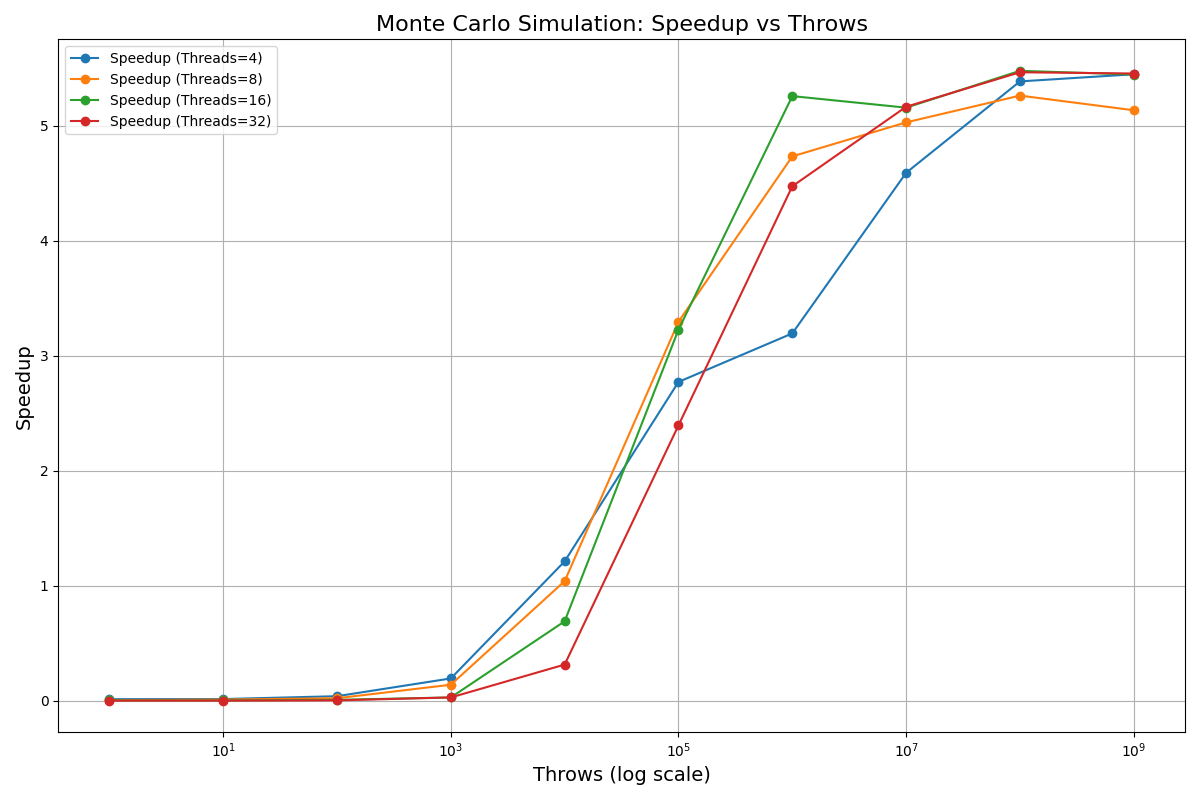
\includegraphics[width=1\textwidth]{monte_carlo_results.png}
    \caption{Χρόνος Εκτέλεσης ανά Αριθμό Νημάτων}
\end{figure}
\subsection*{Συμπεράσματα}
\begin{enumerate}
    \item Ο συγχρονισμός εξασφαλίζει ορθά αποτελέσματα, αλλά προσθέτει overhead.
    \item Η παράλληλη υλοποίηση είναι αποδοτική για μεγάλες εισόδους.
    \item Ο αριθμός πυρήνων περιορίζει την κλιμάκωση της επιτάχυνσης.
\end{enumerate}
Με την ανάλυση αυτή, αποδείξαμε τη χρησιμότητα της παράλληλης μεθόδου Monte Carlo και αναδείξαμε τη σημασία του συγχρονισμού για ακριβή αποτελέσματα.
\section*{Άσκηση 1.2}
\subsection*{Εισαγωγή}
Ο στόχος της άσκησης είναι η υλοποίηση ενός προγράμματος με τη χρήση της βιβλιοθήκης Pthreads, όπου πολλαπλά νήματα ενημερώνουν μία κοινόχρηστη μεταβλητή. Υλοποιήθηκαν δύο προσεγγίσεις για τη διασφάλιση της ορθής εκτέλεσης:
\begin{enumerate}
    \item Με χρήση \textbf{pthread κλειδώματος (mutex locks)}.
    \item Με χρήση \textbf{ατομικών εντολών (atomic operations)}.
\end{enumerate}
Για κάθε προσέγγιση εξετάσαμε την απόδοση με διαφορετικό αριθμό νημάτων και σχολιάσαμε τις διαφορές.
\subsection*{Συγχρονισμός}
Για την αποφυγή συνθηκών ανταγωνισμού (race conditions) κατά την ενημέρωση της κοινόχρηστης μεταβλητής:
\begin{enumerate}
    \item Στην πρώτη προσέγγιση (\path{increase.c}) χρησιμοποιήσαμε \textbf{pthread mutex locks}.
    \item Στη δεύτερη προσέγγιση (\path{increase_atomic.c}) χρησιμοποιήσαμε \textbf{ατομικές εντολές}, μέσω της βιβλιοθήκης \path{stdatomic.h}, και την εντολή \path{atomic_fetch_add} για ασφαλή πρόσβαση στη μεταβλητή.
\end{enumerate}

\subsection*{Πειραματική Διαδικασία}
\begin{itemize} 
    \item \textbf{Παραμετροποίηση:} 
    \begin{itemize} 
        \item Αριθμός νημάτων: 1, 2, 4, 8, 16, 32. 
        \item Συνολικές επαναλήψεις: $34,100,654,080$. 
    \end{itemize} 
    \item \textbf{Εκτέλεση:} 
    \begin{itemize} 
        \item Κάθε πείραμα εκτελέστηκε 5 φορές. 
        \item Τα αποτελέσματα αποθηκεύτηκαν σε αρχείο CSV. 
    \end{itemize} 
    \item \textbf{Αυτοματοποίηση:} 
    \begin{itemize} 
        \item Αναπτύξαμε Python scripts για την εκτέλεση των πειραμάτων και την καταγραφή των δεδομένων.
        \item Χρησιμοποιήσαμε Python scripts για την ανάλυση των δεδομένων και τη δημιουργία γραφημάτων.
    \end{itemize} 
\end{itemize}
\subsection*{Αποτελέσματα}
Τα αποτελέσματα δείχνουν τις επιδόσεις κάθε προσέγγισης για διαφορετικό αριθμό νημάτων.
\begin{itemize} 
    \item \textbf{Σύγκριση Προσεγγίσεων:} 
    \begin{itemize} 
        \item Η χρήση \textbf{mutex locks} (\path{increase.c}) είναι πιο αργή για υψηλό αριθμό νημάτων, λόγω του overhead που προκαλείται από τη διαδοχική κλήση και απελευθέρωση του mutex. 
        \item Η χρήση \textbf{atomic operations} (\path{increase_atomic.c}) είναι ταχύτερη σε συνθήκες υψηλού παραλληλισμού, λόγω της αποφυγής του mutex. 
    \end{itemize} 
    \item \textbf{Ακρίβεια Αποτελεσμάτων:} 
    \begin{itemize} 
        \item Και οι δύο προσεγγίσεις παρήγαγαν το σωστό αποτέλεσμα ($34,100,654,080$) για όλα τα πειράματα, εξασφαλίζοντας τη λειτουργική ορθότητα. 
    \end{itemize} 
    \item \textbf{Κλιμάκωση:} 
    \begin{itemize} 
        \item Οι επιδόσεις βελτιώθηκαν γραμμικά για την προσέγγιση με atomic operations όσο αυξανόταν ο αριθμός των νημάτων. 
        \item Το mutex παρουσιάζει περιορισμένη κλιμάκωση λόγω αυξημένου synchronization overhead. 
    \end{itemize} 
\end{itemize}
\subsection*{Γραφήματα}
Το παρακάτω γράφημα απεικονίζει τη σχέση μεταξύ αριθμού νημάτων και χρόνου εκτέλεσης:
\begin{figure}[h] 
    \centering 
    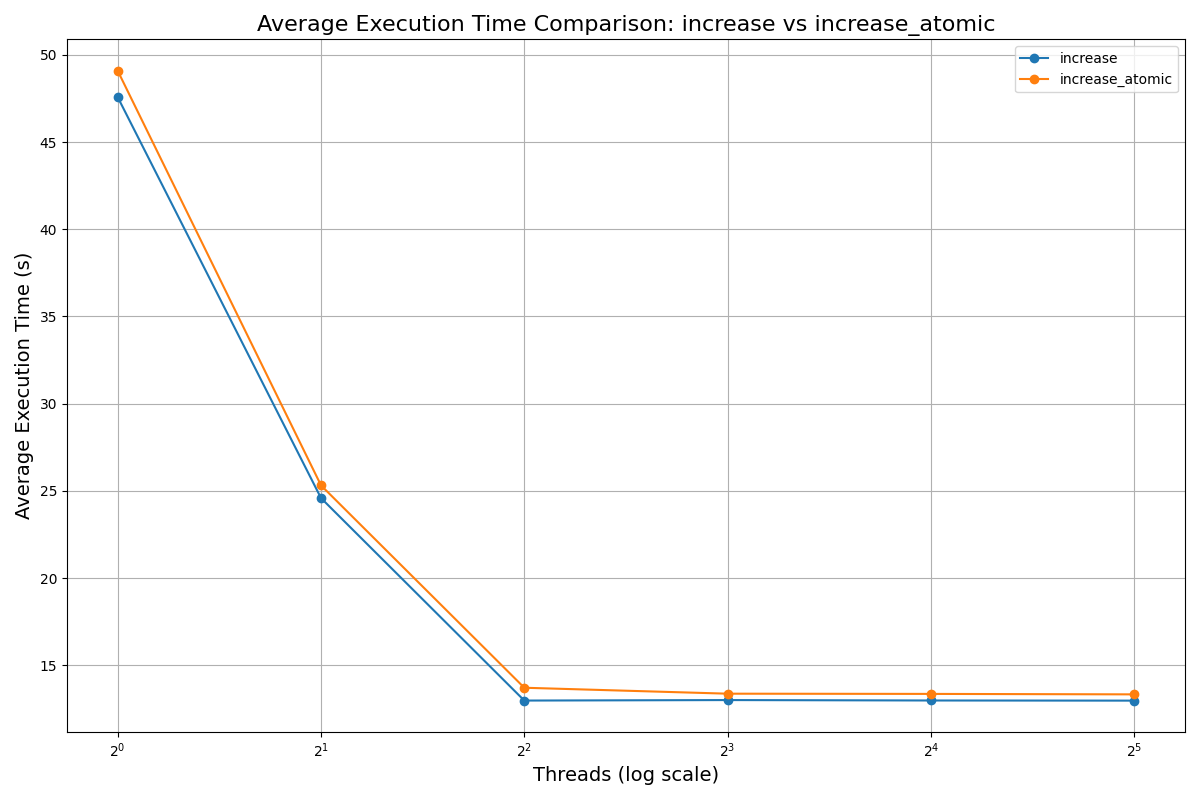
\includegraphics[width=1\textwidth]{increase_results.png} 
    \caption{Χρόνος Εκτέλεσης για τις Προσεγγίσεις Mutex και Atomic} 
\end{figure}
\subsection*{Συμπεράσματα}
\begin{enumerate} 
    \item Η χρήση \textbf{atomic operations} είναι αποδοτικότερη σε συνθήκες παραλληλισμού, καθώς αποφεύγεται το overhead των mutex locks. 
    \item Η μέθοδος με mutex locks παραμένει χρήσιμη για σενάρια με περιορισμένο αριθμό νημάτων. 
    \item Η ακρίβεια των αποτελεσμάτων διασφαλίζεται πλήρως και από τις δύο προσεγγίσεις. 
\end{enumerate} 
Με την ανάλυση αυτή, αποδείξαμε τη σημασία του συγχρονισμού για την αποφυγή συνθηκών ανταγωνισμού και τη δυνατότητα κλιμάκωσης του παραλληλισμού μέσω ατομικών εντολών.
\section*{Άσκηση 1.3}
\subsection*{Εισαγωγή}
Σκοπός της άσκησης είναι η υλοποίηση ενός παράλληλου προγράμματος που χρησιμοποιεί έναν κοινόχρηστο πίνακα για τη διανομή ενημερώσεων μεταξύ των νημάτων. Κάθε νήμα είναι υπεύθυνο για την ενημέρωση ενός στοιχείου του πίνακα, αυξάνοντας την τιμή του. Το πρόγραμμα εξασφαλίζει καθοριστικές τελικές τιμές για τα στοιχεία του πίνακα, καθώς και για το συνολικό άθροισμα. Για να επιτευχθεί αυτό, χρησιμοποιήθηκαν μηχανισμοί συγχρονισμού ώστε να αποφεύγονται συνθήκες ανταγωνισμού (race conditions). Επιπλέον, αναπτύξαμε Python scripts για την αυτοματοποίηση των πειραμάτων και την επεξεργασία των αποτελεσμάτων και τη δημιουργία γραφημάτων.
\subsection*{Συγχρονισμός}
Για να εξασφαλιστούν οι σωστές ενημερώσεις του κοινόχρηστου πίνακα, χρησιμοποιήθηκαν \textbf{mutex locks}. Ο συγχρονισμός ήταν απαραίτητος για την αποφυγή συνθηκών ανταγωνισμού και τη διασφάλιση της ορθότητας των αποτελεσμάτων. Παρόλο που κάθε νήμα ενημερώνει ένα ξεχωριστό στοιχείο, ο συγχρονισμός εξασφαλίζει σωστές προσβάσεις κατά τον υπολογισμό του συνολικού αθροίσματος.
\subsection*{Πειραματική Διαδικασία}
\begin{itemize}
    \item \textbf{Παραμετροποίηση:}
    \begin{itemize}
        \item Αριθμός νημάτων: 1, 2, 4, 8, 16, 32.
        \item Συνολικές ενημερώσεις: 24,100,654,080 επαναλήψεις.
    \end{itemize}
    \item \textbf{Εκτέλεση:}
    \begin{itemize}
        \item Κάθε πείραμα εκτελέστηκε 5 φορές.
        \item Τα αποτελέσματα αποθηκεύτηκαν σε αρχείο CSV.
    \end{itemize}
    \item \textbf{Αυτοματοποίηση:}
    \begin{itemize}
        \item Αναπτύξαμε Python scripts για την εκτέλεση των πειραμάτων και την καταγραφή των δεδομένων.
        \item Χρησιμοποιήσαμε Python scripts για την ανάλυση των δεδομένων και τη δημιουργία γραφημάτων.
    \end{itemize}
\end{itemize}
\subsection*{Αποτελέσματα}
\begin{itemize}
    \item \textbf{Ανάλυση Απόδοσης:}
    \begin{itemize}
        \item Ο χρόνος εκτέλεσης μειώνεται καθώς αυξάνεται ο αριθμός των νημάτων.
        \item Το overhead συγχρονισμού είναι εμφανές όταν ο αριθμός των νημάτων είναι μικρός.
        \item Η απόδοση βελτιώνεται έως ότου ο αριθμός νημάτων φτάσει τον αριθμό των πυρήνων του επεξεργαστή.
    \end{itemize}
    \item \textbf{Επίδραση Συγχρονισμού:}
    \begin{itemize}
        \item Οι σωστές ενημερώσεις του πίνακα είναι εγγυημένες.
        \item Το overhead από τα mutex locks αυξάνεται με τον αριθμό των νημάτων.
    \end{itemize}
\end{itemize}
\subsection*{Γραφήματα}
Το παρακάτω γράφημα δείχνει τον χρόνο εκτέλεσης σε συνάρτηση με τον αριθμό των νημάτων:
\begin{figure}[h]
    \centering
    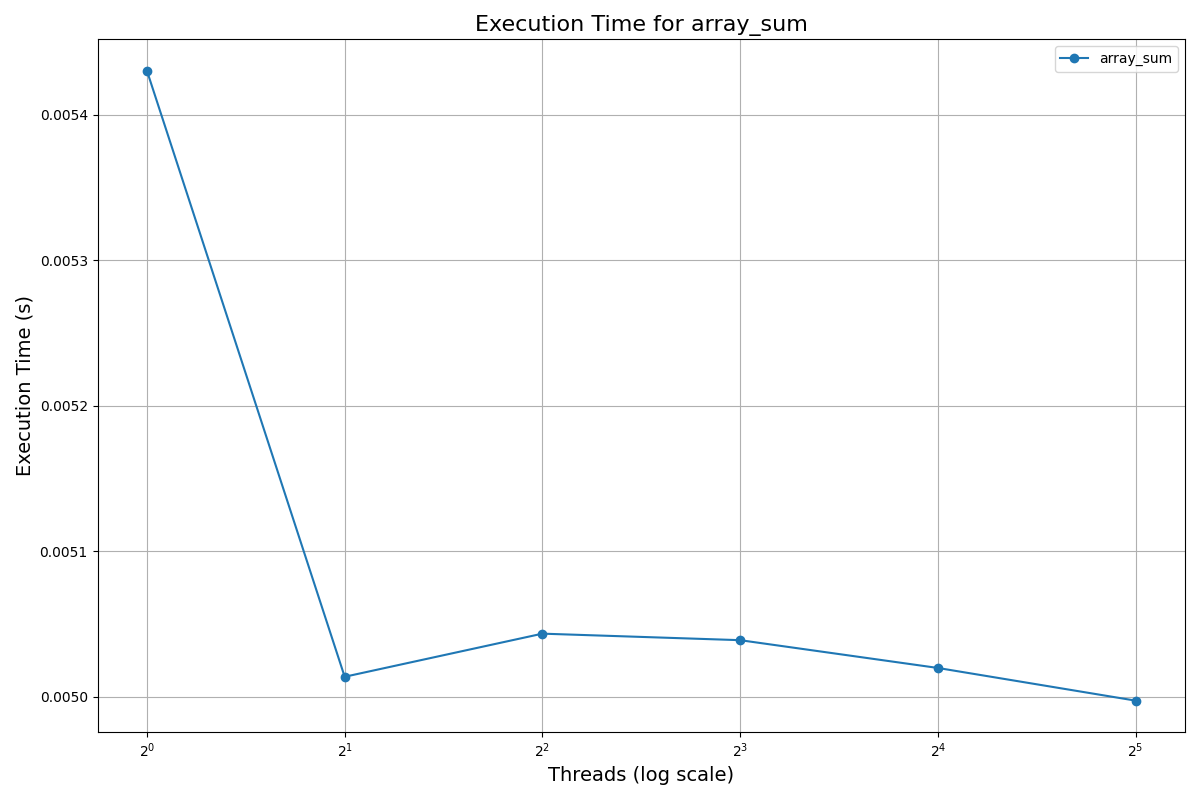
\includegraphics[width=1\textwidth]{array_sum_results.png}
    \caption{Χρόνος Εκτέλεσης ως Συνάρτηση των Νημάτων για την Υλοποίηση \protect\path{array_sum}}
\end{figure}
\subsection*{Συμπεράσματα}
\begin{enumerate}
    \item Ο συγχρονισμός εξασφαλίζει σωστά αποτελέσματα, αλλά προσθέτει overhead.
    \item Η παράλληλη υλοποίηση βελτιώνει σημαντικά την απόδοση για μεγάλες εργασίες.
    \item Η απόδοση περιορίζεται από τον αριθμό των πυρήνων του επεξεργαστή.
    \item Η βελτιστοποίηση της διαχείρισης νημάτων και η μείωση του overhead συγχρονισμού μπορούν να βελτιώσουν περαιτέρω την απόδοση.
\end{enumerate}
Με την ανάλυση αυτή, αποδεικνύεται η χρησιμότητα του παράλληλου προγραμματισμού και η σημασία του συγχρονισμού σε σενάρια κοινόχρηστων δεδομένων.
\section*{Άσκηση 1.4}
\subsection*{Εισαγωγή}
Η παρούσα εργασία αφορά την υλοποίηση και την ανάλυση απόδοσης ενός μηχανισμού κλειδώματος ανάγνωσης-εγγραφής (Reader-Writer Lock). Στόχος ήταν η ανάπτυξη μιας δομής που περιλαμβάνει δύο μεταβλητές συνθήκης (\path{pthread_cond_t}) και ένα mutex (\path{pthread_mutex_t}) για την εξασφάλιση της αμοιβαίας αποκλειστικότητας και του συντονισμού μεταξύ νημάτων ανάγνωσης και εγγραφής. Υλοποιήθηκαν και δοκιμάστηκαν δύο πολιτικές προτεραιότητας:
\begin{itemize}
    \item Προτεραιότητα στα νήματα ανάγνωσης.
    \item Προτεραιότητα στα νήματα εγγραφής.
\end{itemize}
\subsection*{Πειραματική Διαδικασία}
Για κάθε πείραμα:
\begin{itemize}
    \item Ο αρχικός κατάλογος περιείχε \textbf{1000 κλειδιά}.
    \item Εκτελέστηκαν \textbf{500,000 λειτουργίες}, με διαφορετικά ποσοστά για τις λειτουργίες:
    \begin{itemize}
        \item 99.9\% / 95\% / 90\% λειτουργίες \textbf{Member()}.
        \item Το υπόλοιπο ποσοστό διαμοιράστηκε σε λειτουργίες \textbf{Insert()} και \textbf{Delete()}.
    \end{itemize}
    \item Εξετάστηκαν οι περιπτώσεις με 2, 4, 8 και 16 νήματα.
    \item Κάθε περίπτωση εκτελέστηκε τόσο με προτεραιότητα στα νήματα ανάγνωσης όσο και στα νήματα εγγραφής.
\end{itemize}
\subsection*{Υλοποίηση}
Η δομή δεδομένων του μηχανισμού κλειδώματος περιλάμβανε:
\begin{itemize}
    \item \path{active_readers}: Αριθμός ενεργών νημάτων ανάγνωσης.
    \item \path{waiting_readers}: Αριθμός νημάτων ανάγνωσης σε αναμονή.
    \item \path{active_writers}: Αριθμός ενεργών νημάτων εγγραφής.
    \item \path{waiting_writers}: Αριθμός νημάτων εγγραφής σε αναμονή.
    \item \path{mutex}: Προστασία της δομής με mutex locks.
    \item \path{readers_cond, writers_cond}: Μεταβλητές συνθήκης για τον συγχρονισμό των νημάτων.
\end{itemize}
\subsection*{Αποτελέσματα}
Τα αποτελέσματα δείχνουν:
\begin{itemize}
    \item Με \textbf{προτεραιότητα στα νήματα ανάγνωσης}:
    \begin{itemize}
        \item Ο χρόνος αναμονής των αναγνωστών μειώθηκε σημαντικά.
        \item Παρατηρήθηκε πιθανό \textbf{starvation} για τα νήματα εγγραφής.
    \end{itemize}
    \item Με \textbf{προτεραιότητα στα νήματα εγγραφής}:
    \begin{itemize}
        \item Μειώθηκε ο χρόνος αναμονής των εγγραφέων.
        \item Τα νήματα ανάγνωσης αντιμετώπισαν καθυστερήσεις.
    \end{itemize}
\end{itemize}
\subsection*{Γραφήματα}
Στο παρακάτω γράφημα παρουσιάζεται η σύγκριση των μέσων χρόνων εκτέλεσης για τις διαφορετικές πολιτικές προτεραιότητας και αριθμούς νημάτων:
\newpage
\begin{figure}[h]
    \centering
    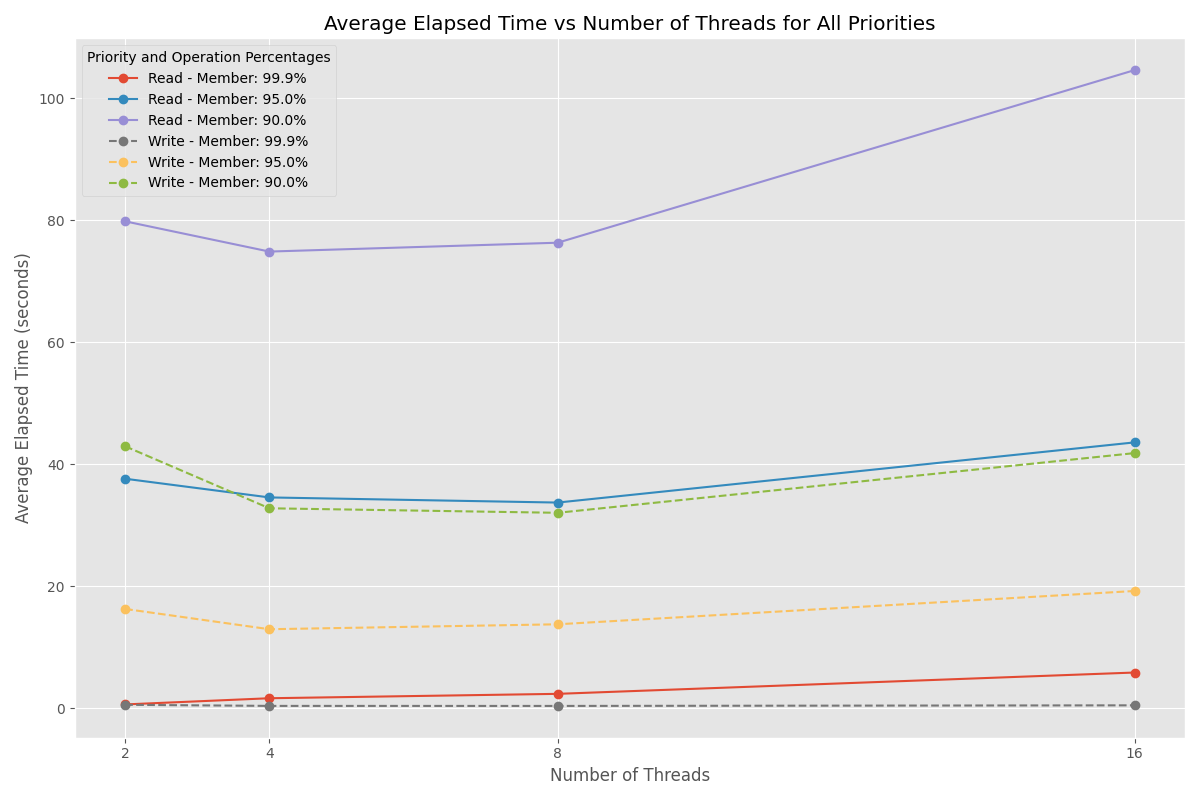
\includegraphics[width=1\textwidth]{rw_lock_results.png}
    \caption{Μέσος χρόνος εκτέλεσης για λειτουργίες ανάγνωσης και εγγραφής ανά πολιτική προτεραιότητας.}
\end{figure}
\subsection*{Συμπεράσματα}
\begin{itemize}
    \item Η χρήση κλειδωμάτων ανάγνωσης-εγγραφής εξασφαλίζει αποτελεσματική πρόσβαση σε κοινόχρηστους πόρους σε πολυνηματικά περιβάλλοντα.
    \item Η επιλογή της πολιτικής προτεραιότητας επηρεάζει άμεσα την απόδοση και την ισορροπία του συστήματος.
    \item Η προτεραιότητα στα νήματα ανάγνωσης είναι κατάλληλη για περιπτώσεις με περισσότερες λειτουργίες \textbf{Member()}, ενώ η προτεραιότητα στα νήματα εγγραφής εξυπηρετεί εφαρμογές με έντονες τροποποιήσεις δεδομένων.
\end{itemize}
\section*{Άσκηση 1.5}
% Περιεχόμενο Άσκησης 1.5 εδώ (αν υπάρχει)
\end{document}
